\bookchapter{Chapitre 49 : Monter l'environnement de développement — Android Studio et le premier projet}

\chapterintro{Pour bien faire le travail, il faut d'abord aiguiser ses outils. Dans ce chapitre, on monte la « cuisine » : installer Android Studio, faire tourner l'émulateur, créer ton tout premier projet Android, puis démonter la structure du projet pour bien la comprendre. Une fois l'environnement prêt, tu verras pour la première fois ton code se transformer en un bouton cliquable — un instant que beaucoup gardent en mémoire toute leur vie.}

\booksection{Installer Android Studio}

Android Studio est l'environnement de développement intégré (IDE) officiel de Google : gratuit, et avec la panoplie complète — écrire du code, prévisualiser l'interface, déboguer, générer le paquet, tout s'y trouve. Quatre étapes pour l'installer :

\begin{enumerate}
  \item Ouvre le site officiel developer.android.com/studio et télécharge la dernière version stable (en août 2026, une version postérieure à Narwhal ; disponible pour Windows/Mac/Linux) ;
  \item lance le programme d'installation et clique sur « Suivant » jusqu'au bout — l'assistant installe automatiquement le SDK Android et les composants de l'émulateur ;
  \item au premier lancement, télécharge les composants du SDK comme indiqué (garde les cases par défaut ; prévois quelques minutes et plusieurs Go d'espace) ;
  \item à la fin, tu arrives sur la page d'accueil — félicitations, la « cuisine » est montée.
\end{enumerate}

\begin{tcbwarn}{Attention : garde en tête la configuration requise}
Android Studio est un grand mangeur de mémoire : 16 Go de RAM recommandés pour bien démarrer (8 Go suffisent pour tourner, mais l'émulateur sera un peu lent), réserve plus de 20 Go de disque et vérifie que le processeur prend en charge la virtualisation (active VT-x/AMD-V dans le BIOS). Si ton ordinateur est vraiment ancien, tu peux remplacer l'émulateur par le « débogage sur appareil réel » (expliqué en section 4 de ce chapitre) : l'expérience en sera même plus fluide.

\end{tcbwarn}

\booksection{Créer ton premier projet}

Sur la page d'accueil, clique sur New Project, choisis le modèle Empty Activity (le plus épuré pour les débutants), puis remplis trois choses :

\begin{center}
\begin{tabularx}{\linewidth}{|X|X|X|}
\hline
\textbf{Champ de configuration} & \textbf{Quoi remplir} & \textbf{Explication} \tabularnewline
\hline
Name & My First App & Le nom de l'app, affiché sur l'écran d'accueil du téléphone \tabularnewline
Package name & com.example.myfirstapp & Identifiant unique au monde ; l'habitude veut qu'on inverse un nom de domaine — garde la valeur par défaut pour l'instant \tabularnewline
Minimum SDK & API 26(Android 8.0) & Version minimale prise en charge, couvrant plus de 95 \% des appareils \tabularnewline
\hline
\end{tabularx}
\end{center}

\begin{center}\small\color{gray}Les trois choses à remplir à la création du projet\end{center}

Après avoir cliqué sur Finish, Android Studio télécharge automatiquement les dépendances et construit le projet avec Gradle (compte quelques minutes la première fois, ce sera bien plus rapide ensuite). Une fois la construction terminée, tu as une app qui tourne — même si elle n'affiche encore qu'un simple « Hello Android! ».

\begin{tcbinfo}{Petit conseil : les subtilités du nom de package}
Le nom de package (package name) est comme le « numéro de carte d'identité » de l'app : il doit être unique dans le monde entier et ne peut plus être changé après publication. Pour t'exercer, com.example.xxx suffit ; pour un vrai produit, remplace-le par ton propre domaine inversé (par exemple com.tonnom.nomdelapp). Ne publie jamais avec com.example — la boutique refuserait l'app.

\end{tcbinfo}

\booksection{Faire tourner : émulateur et appareil réel}

Le code est écrit, il faut maintenant un « téléphone » pour le faire tourner. Tu as deux options :

\booksubsection{L'émulateur (Emulator)}

L'émulateur crée un téléphone Android virtuel dans ton ordinateur. Dans Android Studio, ouvre Device Manager > Create Device, choisis un appareil (les Pixel sont recommandés), sélectionne une image système (avec les Google APIs), télécharge-la, puis démarre-la. Clique ensuite sur le triangle vert Run de la barre d'outils : quelques secondes plus tard, ton app apparaît sur l'écran du « téléphone ».

\booksubsection{Le débogage sur appareil réel (encore mieux)}

Un appareil réel reste l'environnement de test le plus authentique — la sensation du tactile, un vrai réseau, de vrais capteurs : l'émulateur ne peut pas rivaliser. Le débogage sur un téléphone Android est tout simple :

\begin{enumerate}
  \item Sur le téléphone, ouvre [Réglages] > [À propos du téléphone] et tape 7 fois de suite sur « Numéro de version » pour activer les « Options développeur » ;
  \item dans [Options développeur], active le débogage USB ;
  \item relie le téléphone à l'ordinateur avec un câble USB et choisis « Autoriser le débogage USB » dans la fenêtre qui s'affiche ;
  \item retourne dans Android Studio : ton téléphone apparaît dans la liste déroulante des appareils de la barre d'outils ; clique sur Run.
\end{enumerate}

\textbf{Piège à éviter : ne laisse pas le débogage USB activé en permanence}\par

Le débogage USB équivaut à ouvrir une « porte dérobée » à l'ordinateur. Quand tu charges ton téléphone dans un lieu public ou que tu le branches sur un ordinateur dont tu n'es pas sûr, désactive toujours le débogage USB pour empêcher quiconque de lire tes données par ce biais. Prends l'habitude de le couper dès la session de développement terminée.

\booksection{Anatomie du projet : à quoi sert chaque fichier}

En ouvrant un projet pour la première fois, l'arborescence de fichiers à gauche peut donner le vertige. Pas de panique : au quotidien, tu passeras 90 \% de ton temps avec ces seuls éléments :

\begin{center}
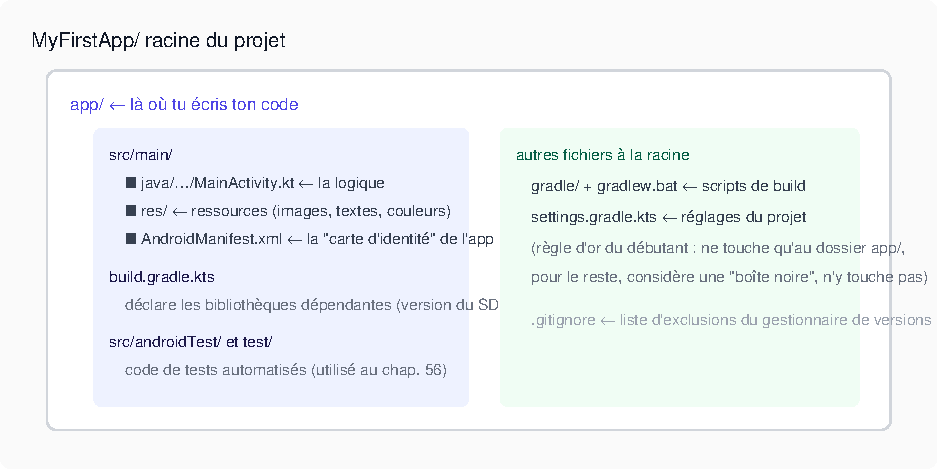
\includegraphics[width=0.92\linewidth]{figures/fig-di-si-shi-jiu-zhang-1}
\\[2pt]\small Figure 2 : la structure du projet que tout débutant doit connaître (règle d'or : ne touche qu'au dossier app/)
\end{center}

\begin{itemize}
  \item MainActivity.kt : la « porte d'entrée » de l'app. Quand l'utilisateur touche l'icône, c'est elle qui est réveillée en premier. Dans le modèle actuel, elle se charge d'afficher « Hello Android! ».
  \item AndroidManifest.xml : le « livret de famille » de l'app — il déclare le nom de l'app, son icône, ses écrans et les permissions nécessaires (appareil photo, localisation, etc.).
  \item Le dossier res/ : l'entrepôt de ressources, où sont rangées images, icônes, textes et couleurs. Placer les textes dans les fichiers de ressources plutôt qu'en dur dans le code est une bonne pratique Android (pratique pour changer de langue ou de thème).
  \item build.gradle.kts : la recette de construction — elle déclare la version minimale prise en charge et les bibliothèques dont le projet dépend (Compose, par exemple).
\end{itemize}

\booksection{Premier essai : remplace « Hello » par ton prénom}

Ouvre MainActivity.kt : tu verras le code généré par le modèle Compose. Trouve la ligne Text(“Hello Android!”), remplace le texte entre guillemets par ton prénom, par exemple Text(“Salut, Jean Dupont ! C'est ma première app”), puis relance avec Ctrl+R (Cmd+R sur Mac). Quelques secondes plus tard, ton prénom s'affiche sur l'émulateur.

\begin{lstlisting}[language=Kotlin]
setContent {
    MyFirstAppTheme {
        Surface(modifier = Modifier.fillMaxSize()) {
            // v remplace ici par ton propre texte
            Text("Bonjour Léa ! Voici ma première app")
        }
    }
}
\end{lstlisting}

Félicitations : tu viens de boucler un cycle complet « modifier le code compiler installer exécuter ». Ce cycle, c'est le quotidien du développeur pour tous les jours à venir. Tant que le fer est chaud, essaie d'autres modifications : agrandis la taille du texte, change la couleur — le chapitre suivant t'expliquera d'où viennent ces « magies ».

\booksection{Premiers secours contre les erreurs fréquentes : les « urgences » des deux premières semaines}

Pendant l'installation de l'environnement et la première construction, tu rencontreras très probablement les trois erreurs suivantes. Pas de panique, chacune a son remède :

\begin{center}
\begin{tabularx}{\linewidth}{|X|X|X|}
\hline
\textbf{Symptôme de l'erreur} & \textbf{Cause fréquente} & \textbf{Remède} \tabularnewline
\hline
Gradle sync failed / téléchargement lent des dépendances & Accès réseau aux dépôts difficile & Configure un dépôt miroir chinois pour Gradle (miroirs maven d'Alibaba Cloud ou de Tencent Cloud) ; cherche « gradle miroir chinois » sur Internet et suis les instructions \tabularnewline
Composants du SDK manquants & Le téléchargement du SDK a été ignoré lors de l'installation & Complète les plateformes et outils manquants via Settings > SDK Manager \tabularnewline
L'émulateur ne démarre pas / écran noir & Virtualisation non activée, image corrompue & Active VT-x/AMD-V dans le BIOS ; supprime l'émulateur et recrée-le ; ou passe directement au débogage sur appareil réel \tabularnewline
\hline
\end{tabularx}
\end{center}

\begin{center}\small\color{gray}Table de secours des erreurs d'environnement pour débutants\end{center}

\begin{tcbinfo}{Petit conseil : la méthode pour chercher une erreur}
La première ligne du message d'erreur est la plus précieuse — copie-la telle quelle dans un moteur de recherche en ajoutant le mot-clé « android studio ». Ne cherche pas des questions vagues du genre « je n'arrive pas à installer mon environnement » ; cherche l'erreur précise, du type « Gradle sync failed: Could not resolve com.android.tools.build ». Aux questions précises, les réponses précises.

\end{tcbinfo}

\begin{tcbpractice}{À toi de jouer : accomplis ta liste de « rituel de développeur »}
(1) Installe Android Studio et fais tourner l'émulateur ; (2) exécute ton app une fois sur un appareil réel et garde une capture d'écran en souvenir ; (3) remplace le texte Hello par ton prénom ; (4) compresse le projet et archive-le. Après ces quatre étapes, tu pourras annoncer à tes amis : moi aussi je suis développeur Android (capture d'écran à l'appui).

\end{tcbpractice}

\begin{tcbsummary}{Résumé du chapitre}
\begin{itemize}
  \item Android Studio = l'IDE officiel gratuit ; recommandé : 16 Go de RAM + 20 Go de disque + virtualisation activée
  \item Les trois clés d'un nouveau projet : le nom, le nom de package (unique au monde, ne publie pas avec com.example) et le SDK minimal (à partir de l'API 26)
  \item Deux façons d'exécuter : l'émulateur (téléphone virtuel dans l'ordinateur) et l'appareil réel (active le débogage USB, pense à le couper ensuite)
  \item Règle d'or du projet : ne touche qu'au dossier app/ — MainActivity.kt est la porte d'entrée, le Manifest le livret de famille, res/ l'entrepôt de ressources
  \item Le quotidien du développeur = modifier le code Run observer le résultat, encore et encore
\end{itemize}

\end{tcbsummary}
